\documentclass[1p]{elsarticle_modified}
%\bibliographystyle{elsarticle-num}

%\usepackage[colorlinks]{hyperref}
%\usepackage{abbrmath_seonhwa} %\Abb, \Ascr, \Acal ,\Abf, \Afrak
\usepackage{amsfonts}
\usepackage{amssymb}
\usepackage{amsmath}
\usepackage{amsthm}
\usepackage{scalefnt}
\usepackage{amsbsy}
\usepackage{kotex}
\usepackage{caption}
\usepackage{subfig}
\usepackage{color}
\usepackage{graphicx}
\usepackage{xcolor} %% white, black, red, green, blue, cyan, magenta, yellow
\usepackage{float}
\usepackage{setspace}
\usepackage{hyperref}

\usepackage{tikz}
\usetikzlibrary{arrows}

\usepackage{multirow}
\usepackage{array} % fixed length table
\usepackage{hhline}

%%%%%%%%%%%%%%%%%%%%%
\makeatletter
\renewcommand*\env@matrix[1][\arraystretch]{%
	\edef\arraystretch{#1}%
	\hskip -\arraycolsep
	\let\@ifnextchar\new@ifnextchar
	\array{*\c@MaxMatrixCols c}}
\makeatother %https://tex.stackexchange.com/questions/14071/how-can-i-increase-the-line-spacing-in-a-matrix
%%%%%%%%%%%%%%%

\usepackage[normalem]{ulem}

\newcommand{\msout}[1]{\ifmmode\text{\sout{\ensuremath{#1}}}\else\sout{#1}\fi}
%SOURCE: \msout is \stkout macro in https://tex.stackexchange.com/questions/20609/strikeout-in-math-mode

\newcommand{\cancel}[1]{
	\ifmmode
	{\color{red}\msout{#1}}
	\else
	{\color{red}\sout{#1}}
	\fi
}

\newcommand{\add}[1]{
	{\color{blue}\uwave{#1}}
}

\newcommand{\replace}[2]{
	\ifmmode
	{\color{red}\msout{#1}}{\color{blue}\uwave{#2}}
	\else
	{\color{red}\sout{#1}}{\color{blue}\uwave{#2}}
	\fi
}

\newcommand{\Sol}{\mathcal{S}} %segment
\newcommand{\D}{D} %diagram
\newcommand{\A}{\mathcal{A}} %arc


%%%%%%%%%%%%%%%%%%%%%%%%%%%%%5 test

\def\sl{\operatorname{\textup{SL}}(2,\Cbb)}
\def\psl{\operatorname{\textup{PSL}}(2,\Cbb)}
\def\quan{\mkern 1mu \triangleright \mkern 1mu}

\theoremstyle{definition}
\newtheorem{thm}{Theorem}[section]
\newtheorem{prop}[thm]{Proposition}
\newtheorem{lem}[thm]{Lemma}
\newtheorem{ques}[thm]{Question}
\newtheorem{cor}[thm]{Corollary}
\newtheorem{defn}[thm]{Definition}
\newtheorem{exam}[thm]{Example}
\newtheorem{rmk}[thm]{Remark}
\newtheorem{alg}[thm]{Algorithm}

\newcommand{\I}{\sqrt{-1}}
\begin{document}

%\begin{frontmatter}
%
%\title{Boundary parabolic representations of knots up to 8 crossings}
%
%%% Group authors per affiliation:
%\author{Yunhi Cho} 
%\address{Department of Mathematics, University of Seoul, Seoul, Korea}
%\ead{yhcho@uos.ac.kr}
%
%
%\author{Seonhwa Kim} %\fnref{s_kim}}
%\address{Center for Geometry and Physics, Institute for Basic Science, Pohang, 37673, Korea}
%\ead{ryeona17@ibs.re.kr}
%
%\author{Hyuk Kim}
%\address{Department of Mathematical Sciences, Seoul National University, Seoul 08826, Korea}
%\ead{hyukkim@snu.ac.kr}
%
%\author{Seokbeom Yoon}
%\address{Department of Mathematical Sciences, Seoul National University, Seoul, 08826,  Korea}
%\ead{sbyoon15@snu.ac.kr}
%
%\begin{abstract}
%We find all boundary parabolic representation of knots up to 8 crossings.
%
%\end{abstract}
%\begin{keyword}
%    \MSC[2010] 57M25 
%\end{keyword}
%
%\end{frontmatter}

%\linenumbers
%\tableofcontents
%
\newcommand\colored[1]{\textcolor{white}{\rule[-0.35ex]{0.8em}{1.4ex}}\kern-0.8em\color{red} #1}%
%\newcommand\colored[1]{\textcolor{white}{ #1}\kern-2.17ex	\textcolor{white}{ #1}\kern-1.81ex	\textcolor{white}{ #1}\kern-2.15ex\color{red}#1	}

{\Large $\underline{12a_{1007}~(K12a_{1007})}$}

\setlength{\tabcolsep}{10pt}
\renewcommand{\arraystretch}{1.6}
\vspace{1cm}\begin{tabular}{m{100pt}>{\centering\arraybackslash}m{274pt}}
\multirow{5}{120pt}{
	\centering
	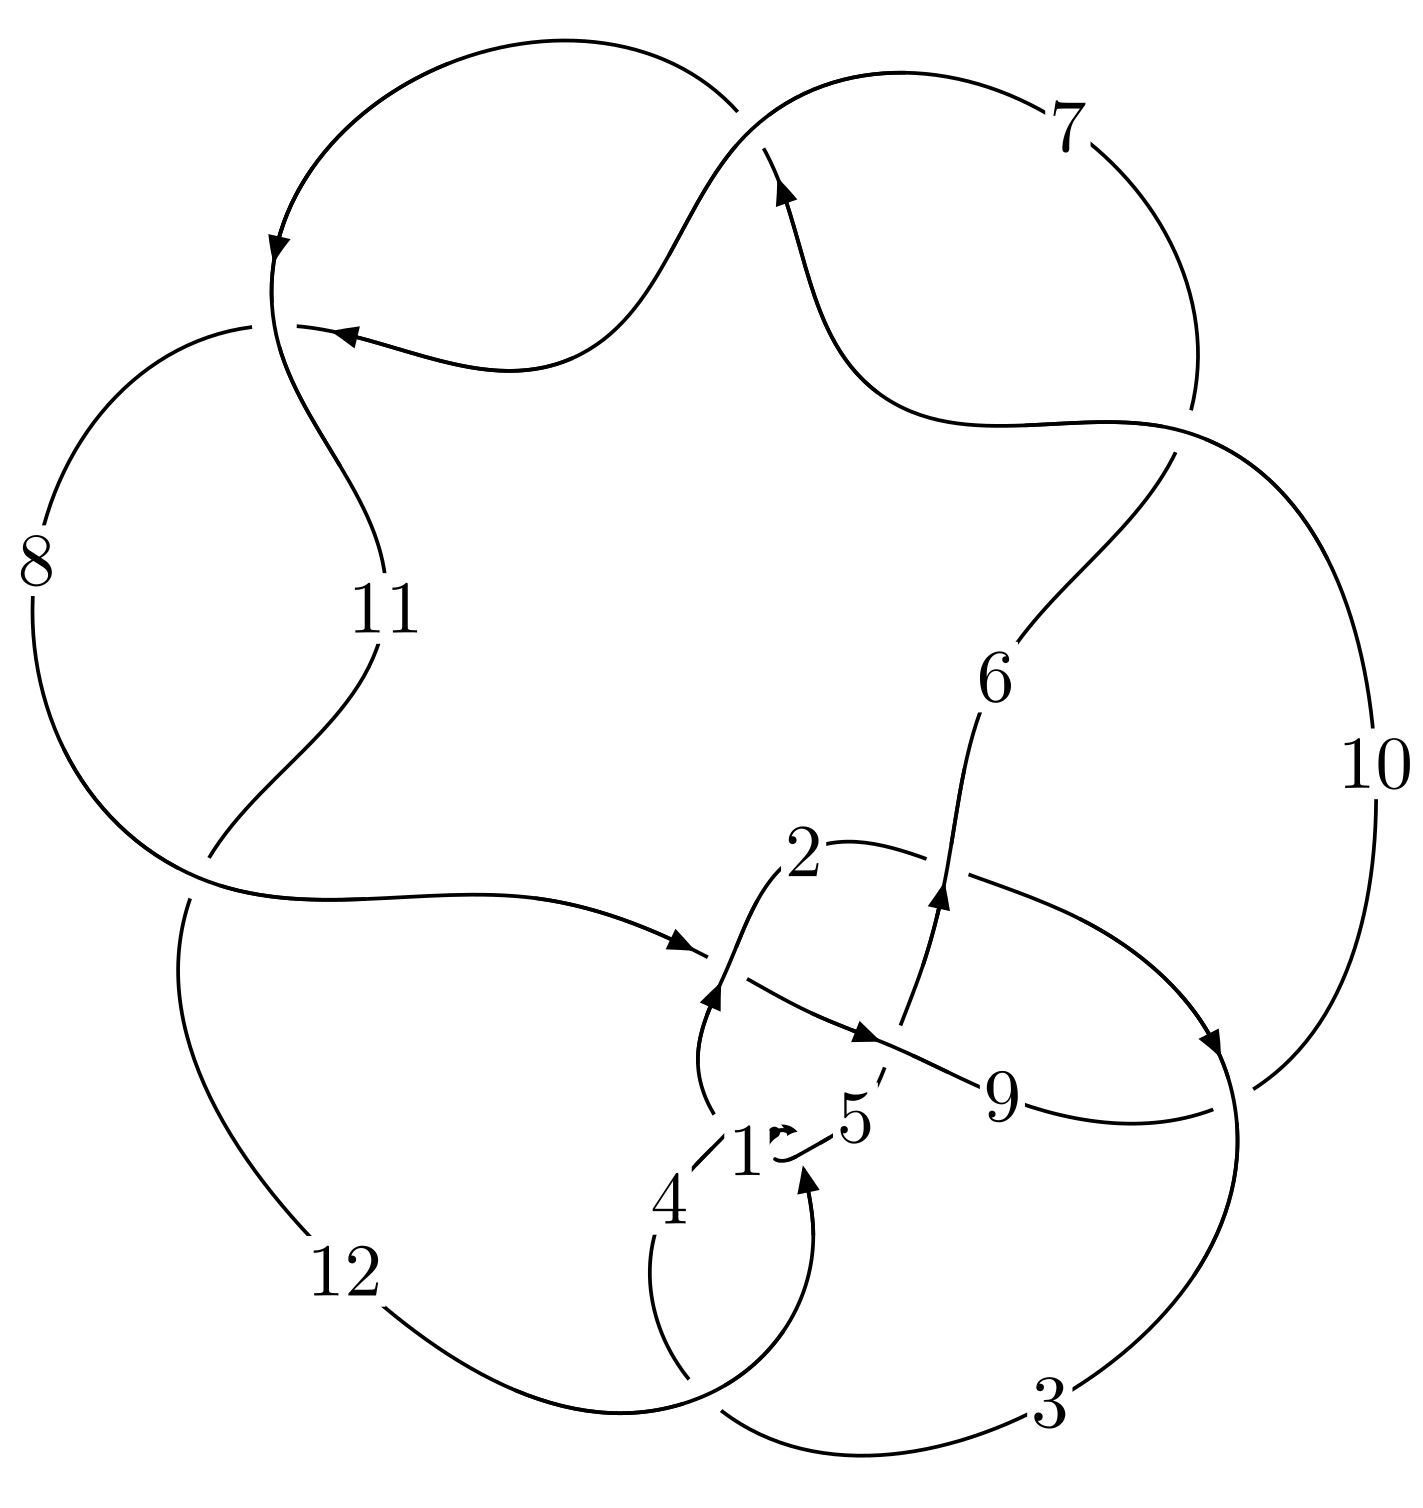
\includegraphics[width=112pt]{../../../GIT/diagram.site/Diagrams/png/1808_12a_1007.png}\\
\ \ \ A knot diagram\footnotemark}&
\allowdisplaybreaks
\textbf{Linearized knot diagam} \\
\cline{2-2}
 &
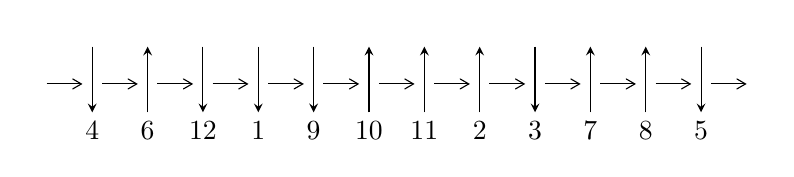
\begin{tikzpicture}[x=20pt, y=17pt]
	% nodes
	\node (C0) at (0, 0) {};
	\node (C1) at (1, 0) {};
	\node (C1U) at (1, +1) {};
	\node (C1D) at (1, -1) {4};

	\node (C2) at (2, 0) {};
	\node (C2U) at (2, +1) {};
	\node (C2D) at (2, -1) {6};

	\node (C3) at (3, 0) {};
	\node (C3U) at (3, +1) {};
	\node (C3D) at (3, -1) {12};

	\node (C4) at (4, 0) {};
	\node (C4U) at (4, +1) {};
	\node (C4D) at (4, -1) {1};

	\node (C5) at (5, 0) {};
	\node (C5U) at (5, +1) {};
	\node (C5D) at (5, -1) {9};

	\node (C6) at (6, 0) {};
	\node (C6U) at (6, +1) {};
	\node (C6D) at (6, -1) {10};

	\node (C7) at (7, 0) {};
	\node (C7U) at (7, +1) {};
	\node (C7D) at (7, -1) {11};

	\node (C8) at (8, 0) {};
	\node (C8U) at (8, +1) {};
	\node (C8D) at (8, -1) {2};

	\node (C9) at (9, 0) {};
	\node (C9U) at (9, +1) {};
	\node (C9D) at (9, -1) {3};

	\node (C10) at (10, 0) {};
	\node (C10U) at (10, +1) {};
	\node (C10D) at (10, -1) {7};

	\node (C11) at (11, 0) {};
	\node (C11U) at (11, +1) {};
	\node (C11D) at (11, -1) {8};

	\node (C12) at (12, 0) {};
	\node (C12U) at (12, +1) {};
	\node (C12D) at (12, -1) {5};
	\node (C13) at (13, 0) {};

	% arrows
	\draw[->,>={angle 60}]
	(C0) edge (C1) (C1) edge (C2) (C2) edge (C3) (C3) edge (C4) (C4) edge (C5) (C5) edge (C6) (C6) edge (C7) (C7) edge (C8) (C8) edge (C9) (C9) edge (C10) (C10) edge (C11) (C11) edge (C12) (C12) edge (C13) ;	\draw[->,>=stealth]
	(C1U) edge (C1D) (C2D) edge (C2U) (C3U) edge (C3D) (C4U) edge (C4D) (C5U) edge (C5D) (C6D) edge (C6U) (C7D) edge (C7U) (C8D) edge (C8U) (C9U) edge (C9D) (C10D) edge (C10U) (C11D) edge (C11U) (C12U) edge (C12D) ;
	\end{tikzpicture} \\
\hhline{~~} \\& 
\textbf{Solving Sequence} \\ \cline{2-2} 
 &
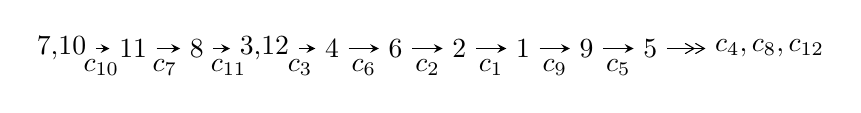
\begin{tikzpicture}[x=23pt, y=7pt]
	% node
	\node (A0) at (-1/8, 0) {7,10};
	\node (A1) at (1, 0) {11};
	\node (A2) at (2, 0) {8};
	\node (A3) at (49/16, 0) {3,12};
	\node (A4) at (33/8, 0) {4};
	\node (A5) at (41/8, 0) {6};
	\node (A6) at (49/8, 0) {2};
	\node (A7) at (57/8, 0) {1};
	\node (A8) at (65/8, 0) {9};
	\node (A9) at (73/8, 0) {5};
	\node (C1) at (1/2, -1) {$c_{10}$};
	\node (C2) at (3/2, -1) {$c_{7}$};
	\node (C3) at (5/2, -1) {$c_{11}$};
	\node (C4) at (29/8, -1) {$c_{3}$};
	\node (C5) at (37/8, -1) {$c_{6}$};
	\node (C6) at (45/8, -1) {$c_{2}$};
	\node (C7) at (53/8, -1) {$c_{1}$};
	\node (C8) at (61/8, -1) {$c_{9}$};
	\node (C9) at (69/8, -1) {$c_{5}$};
	\node (A10) at (11, 0) {$c_{4},c_{8},c_{12}$};

	% edge
	\draw[->,>=stealth]	
	(A0) edge (A1) (A1) edge (A2) (A2) edge (A3) (A3) edge (A4) (A4) edge (A5) (A5) edge (A6) (A6) edge (A7) (A7) edge (A8) (A8) edge (A9) ;
	\draw[->>,>={angle 60}]	
	(A9) edge (A10);
\end{tikzpicture} \\ 

\end{tabular} \\

\footnotetext{
The image of knot diagram is generated by the software ``\textbf{Draw programme}" developed by Andrew Bartholomew(\url{http://www.layer8.co.uk/maths/draw/index.htm\#Running-draw}), where we modified some parts for our purpose(\url{https://github.com/CATsTAILs/LinksPainter}).
}\phantom \\ \newline 
\centering \textbf{Ideals for irreducible components\footnotemark of $X_{\text{par}}$} 
 
\begin{align*}
I^u_{1}&=\langle 
-2.73105\times10^{74} u^{73}+1.04551\times10^{75} u^{72}+\cdots+6.63560\times10^{73} b+5.79542\times10^{74},\\
\phantom{I^u_{1}}&\phantom{= \langle  }2.90380\times10^{74} u^{73}-1.11784\times10^{75} u^{72}+\cdots+6.63560\times10^{73} a-7.84843\times10^{74},\;u^{74}-4 u^{73}+\cdots+3 u+1\rangle \\
I^u_{2}&=\langle 
b+a,\;a^3+a^2-1,\;u-1\rangle \\
\\
\end{align*}
\raggedright * 2 irreducible components of $\dim_{\mathbb{C}}=0$, with total 77 representations.\\
\footnotetext{All coefficients of polynomials are rational numbers. But the coefficients are sometimes approximated in decimal forms when there is not enough margin.}
\newpage
\renewcommand{\arraystretch}{1}
\centering \section*{I. $I^u_{1}= \langle -2.73\times10^{74} u^{73}+1.05\times10^{75} u^{72}+\cdots+6.64\times10^{73} b+5.80\times10^{74},\;2.90\times10^{74} u^{73}-1.12\times10^{75} u^{72}+\cdots+6.64\times10^{73} a-7.85\times10^{74},\;u^{74}-4 u^{73}+\cdots+3 u+1 \rangle$}
\flushleft \textbf{(i) Arc colorings}\\
\begin{tabular}{m{7pt} m{180pt} m{7pt} m{180pt} }
\flushright $a_{7}=$&$\begin{pmatrix}0\\u\end{pmatrix}$ \\
\flushright $a_{10}=$&$\begin{pmatrix}1\\0\end{pmatrix}$ \\
\flushright $a_{11}=$&$\begin{pmatrix}1\\- u^2\end{pmatrix}$ \\
\flushright $a_{8}=$&$\begin{pmatrix}u\\- u^3+u\end{pmatrix}$ \\
\flushright $a_{3}=$&$\begin{pmatrix}-4.37609 u^{73}+16.8460 u^{72}+\cdots+52.4768 u+11.8278\\4.11576 u^{73}-15.7560 u^{72}+\cdots-45.0010 u-8.73384\end{pmatrix}$ \\
\flushright $a_{12}=$&$\begin{pmatrix}- u^2+1\\u^4-2 u^2\end{pmatrix}$ \\
\flushright $a_{4}=$&$\begin{pmatrix}-6.70751 u^{73}+23.6093 u^{72}+\cdots+56.6250 u+12.6818\\7.05505 u^{73}-24.6502 u^{72}+\cdots-59.0346 u-11.9969\end{pmatrix}$ \\
\flushright $a_{6}=$&$\begin{pmatrix}- u\\u\end{pmatrix}$ \\
\flushright $a_{2}=$&$\begin{pmatrix}-5.25069 u^{73}+18.6857 u^{72}+\cdots+52.3624 u+11.8764\\4.99036 u^{73}-17.5957 u^{72}+\cdots-44.8866 u-8.78248\end{pmatrix}$ \\
\flushright $a_{1}=$&$\begin{pmatrix}6.92512 u^{73}-21.5547 u^{72}+\cdots-40.4571 u-7.72040\\-6.48591 u^{73}+20.1000 u^{72}+\cdots+34.5039 u+7.98169\end{pmatrix}$ \\
\flushright $a_{9}=$&$\begin{pmatrix}3.64853 u^{73}-11.8343 u^{72}+\cdots-31.7013 u-7.77982\\-6.07450 u^{73}+18.8967 u^{72}+\cdots+44.3898 u+8.64309\end{pmatrix}$ \\
\flushright $a_{5}=$&$\begin{pmatrix}1.21712 u^{73}-5.23446 u^{72}+\cdots-18.5691 u-4.25242\\-1.21712 u^{73}+5.23446 u^{72}+\cdots+18.5691 u+3.25242\end{pmatrix}$\\&\end{tabular}
\flushleft \textbf{(ii) Obstruction class $= -1$}\\~\\
\flushleft \textbf{(iii) Cusp Shapes $= 90.9880 u^{73}-311.861 u^{72}+\cdots-727.709 u-161.363$}\\~\\
\newpage\renewcommand{\arraystretch}{1}
\flushleft \textbf{(iv) u-Polynomials at the component}\newline \\
\begin{tabular}{m{50pt}|m{274pt}}
Crossings & \hspace{64pt}u-Polynomials at each crossing \\
\hline $$\begin{aligned}c_{1},c_{4},c_{12}\end{aligned}$$&$\begin{aligned}
&u^{74}-2 u^{73}+\cdots+14 u-1
\end{aligned}$\\
\hline $$\begin{aligned}c_{2}\end{aligned}$$&$\begin{aligned}
&u^{74}-5 u^{73}+\cdots-4 u+8
\end{aligned}$\\
\hline $$\begin{aligned}c_{3}\end{aligned}$$&$\begin{aligned}
&u^{74}+2 u^{73}+\cdots+316 u-113
\end{aligned}$\\
\hline $$\begin{aligned}c_{5}\end{aligned}$$&$\begin{aligned}
&u^{74}+4 u^{73}+\cdots-3 u-1
\end{aligned}$\\
\hline $$\begin{aligned}c_{6},c_{7},c_{10}\\c_{11}\end{aligned}$$&$\begin{aligned}
&u^{74}-4 u^{73}+\cdots+3 u+1
\end{aligned}$\\
\hline $$\begin{aligned}c_{8}\end{aligned}$$&$\begin{aligned}
&u^{74}+29 u^{72}+\cdots-10528 u-1472
\end{aligned}$\\
\hline $$\begin{aligned}c_{9}\end{aligned}$$&$\begin{aligned}
&u^{74}+2 u^{73}+\cdots-1674 u+189
\end{aligned}$\\
\hline
\end{tabular}\\~\\
\newpage\renewcommand{\arraystretch}{1}
\flushleft \textbf{(v) Riley Polynomials at the component}\newline \\
\begin{tabular}{m{50pt}|m{274pt}}
Crossings & \hspace{64pt}Riley Polynomials at each crossing \\
\hline $$\begin{aligned}c_{1},c_{4},c_{12}\end{aligned}$$&$\begin{aligned}
&y^{74}+66 y^{73}+\cdots-86 y+1
\end{aligned}$\\
\hline $$\begin{aligned}c_{2}\end{aligned}$$&$\begin{aligned}
&y^{74}-21 y^{73}+\cdots+176 y+64
\end{aligned}$\\
\hline $$\begin{aligned}c_{3}\end{aligned}$$&$\begin{aligned}
&y^{74}-6 y^{73}+\cdots-1391446 y+12769
\end{aligned}$\\
\hline $$\begin{aligned}c_{5}\end{aligned}$$&$\begin{aligned}
&y^{74}-8 y^{73}+\cdots-11 y+1
\end{aligned}$\\
\hline $$\begin{aligned}c_{6},c_{7},c_{10}\\c_{11}\end{aligned}$$&$\begin{aligned}
&y^{74}-88 y^{73}+\cdots-11 y+1
\end{aligned}$\\
\hline $$\begin{aligned}c_{8}\end{aligned}$$&$\begin{aligned}
&y^{74}+58 y^{73}+\cdots-88558592 y+2166784
\end{aligned}$\\
\hline $$\begin{aligned}c_{9}\end{aligned}$$&$\begin{aligned}
&y^{74}+90 y^{73}+\cdots-75006 y+35721
\end{aligned}$\\
\hline
\end{tabular}\\~\\
\newpage\flushleft \textbf{(vi) Complex Volumes and Cusp Shapes}
$$\begin{array}{c|c|c}  
\text{Solutions to }I^u_{1}& \I (\text{vol} + \sqrt{-1}CS) & \text{Cusp shape}\\
 \hline 
\begin{aligned}
u &= -0.942093 + 0.309194 I \\
a &= \phantom{-}0.82178 - 1.53663 I \\
b &= \phantom{-}0.512844 + 1.053040 I\end{aligned}
 & \phantom{-}9.22994 - 3.76689 I & \phantom{-0.000000 } 0 \\ \hline\begin{aligned}
u &= -0.942093 - 0.309194 I \\
a &= \phantom{-}0.82178 + 1.53663 I \\
b &= \phantom{-}0.512844 - 1.053040 I\end{aligned}
 & \phantom{-}9.22994 + 3.76689 I & \phantom{-0.000000 } 0 \\ \hline\begin{aligned}
u &= -0.829214 + 0.539612 I \\
a &= \phantom{-}0.454823 - 1.201050 I \\
b &= \phantom{-}0.93839 + 1.08699 I\end{aligned}
 & \phantom{-}0.17157 - 8.96993 I & \phantom{-0.000000 } 0 \\ \hline\begin{aligned}
u &= -0.829214 - 0.539612 I \\
a &= \phantom{-}0.454823 + 1.201050 I \\
b &= \phantom{-}0.93839 - 1.08699 I\end{aligned}
 & \phantom{-}0.17157 + 8.96993 I & \phantom{-0.000000 } 0 \\ \hline\begin{aligned}
u &= \phantom{-}0.759294 + 0.675735 I \\
a &= -0.727541 - 0.427353 I \\
b &= \phantom{-}0.083007 + 0.966573 I\end{aligned}
 & \phantom{-}6.66017 + 4.10483 I & \phantom{-0.000000 } 0 \\ \hline\begin{aligned}
u &= \phantom{-}0.759294 - 0.675735 I \\
a &= -0.727541 + 0.427353 I \\
b &= \phantom{-}0.083007 - 0.966573 I\end{aligned}
 & \phantom{-}6.66017 - 4.10483 I & \phantom{-0.000000 } 0 \\ \hline\begin{aligned}
u &= -0.875516 + 0.576026 I \\
a &= -0.378694 + 1.296850 I \\
b &= -0.94555 - 1.18981 I\end{aligned}
 & \phantom{-}5.52475 - 12.85780 I & \phantom{-0.000000 } 0 \\ \hline\begin{aligned}
u &= -0.875516 - 0.576026 I \\
a &= -0.378694 - 1.296850 I \\
b &= -0.94555 + 1.18981 I\end{aligned}
 & \phantom{-}5.52475 + 12.85780 I & \phantom{-0.000000 } 0 \\ \hline\begin{aligned}
u &= -0.783161 + 0.448813 I \\
a &= -0.672469 + 1.120440 I \\
b &= -0.846780 - 0.934444 I\end{aligned}
 & \phantom{-}1.93066 - 4.73106 I & \phantom{-0.000000 } 0 \\ \hline\begin{aligned}
u &= -0.783161 - 0.448813 I \\
a &= -0.672469 - 1.120440 I \\
b &= -0.846780 + 0.934444 I\end{aligned}
 & \phantom{-}1.93066 + 4.73106 I & \phantom{-0.000000 } 0\\
 \hline 
 \end{array}$$\newpage$$\begin{array}{c|c|c}  
\text{Solutions to }I^u_{1}& \I (\text{vol} + \sqrt{-1}CS) & \text{Cusp shape}\\
 \hline 
\begin{aligned}
u &= \phantom{-}1.019360 + 0.418934 I \\
a &= -0.652930 - 0.054022 I \\
b &= \phantom{-}0.195417 + 0.497499 I\end{aligned}
 & \phantom{-}1.233780 - 0.643810 I & \phantom{-0.000000 } 0 \\ \hline\begin{aligned}
u &= \phantom{-}1.019360 - 0.418934 I \\
a &= -0.652930 + 0.054022 I \\
b &= \phantom{-}0.195417 - 0.497499 I\end{aligned}
 & \phantom{-}1.233780 + 0.643810 I & \phantom{-0.000000 } 0 \\ \hline\begin{aligned}
u &= \phantom{-}0.683679 + 0.520772 I \\
a &= \phantom{-}0.646846 + 0.414647 I \\
b &= \phantom{-}0.063130 - 0.851636 I\end{aligned}
 & \phantom{-}1.52626 + 1.62659 I & \phantom{-0.000000 } 0 \\ \hline\begin{aligned}
u &= \phantom{-}0.683679 - 0.520772 I \\
a &= \phantom{-}0.646846 - 0.414647 I \\
b &= \phantom{-}0.063130 + 0.851636 I\end{aligned}
 & \phantom{-}1.52626 - 1.62659 I & \phantom{-0.000000 } 0 \\ \hline\begin{aligned}
u &= -0.042815 + 0.820802 I \\
a &= -0.022920 - 0.248405 I \\
b &= \phantom{-}0.752740 - 0.872074 I\end{aligned}
 & \phantom{-}2.99294 + 8.23725 I & \phantom{-0.000000 } 0 \\ \hline\begin{aligned}
u &= -0.042815 - 0.820802 I \\
a &= -0.022920 + 0.248405 I \\
b &= \phantom{-}0.752740 + 0.872074 I\end{aligned}
 & \phantom{-}2.99294 - 8.23725 I & \phantom{-0.000000 } 0 \\ \hline\begin{aligned}
u &= \phantom{-}1.041600 + 0.561025 I \\
a &= \phantom{-}0.843277 + 0.134056 I \\
b &= -0.345412 - 0.645126 I\end{aligned}
 & \phantom{-}6.23102 - 3.52690 I & \phantom{-0.000000 } 0 \\ \hline\begin{aligned}
u &= \phantom{-}1.041600 - 0.561025 I \\
a &= \phantom{-}0.843277 - 0.134056 I \\
b &= -0.345412 + 0.645126 I\end{aligned}
 & \phantom{-}6.23102 + 3.52690 I & \phantom{-0.000000 } 0 \\ \hline\begin{aligned}
u &= \phantom{-}0.804616\phantom{ +0.000000I} \\
a &= \phantom{-}0.0596040\phantom{ +0.000000I} \\
b &= -0.470934\phantom{ +0.000000I}\end{aligned}
 & \phantom{-}1.37963\phantom{ +0.000000I} & \phantom{-}7.78020\phantom{ +0.000000I} \\ \hline\begin{aligned}
u &= \phantom{-}0.278147 + 0.701699 I \\
a &= -0.531426 - 0.183780 I \\
b &= -0.370065 + 0.993896 I\end{aligned}
 & \phantom{-}5.32512 + 0.61066 I & \phantom{-}6.95537 - 3.49676 I\\
 \hline 
 \end{array}$$\newpage$$\begin{array}{c|c|c}  
\text{Solutions to }I^u_{1}& \I (\text{vol} + \sqrt{-1}CS) & \text{Cusp shape}\\
 \hline 
\begin{aligned}
u &= \phantom{-}0.278147 - 0.701699 I \\
a &= -0.531426 + 0.183780 I \\
b &= -0.370065 - 0.993896 I\end{aligned}
 & \phantom{-}5.32512 - 0.61066 I & \phantom{-}6.95537 + 3.49676 I \\ \hline\begin{aligned}
u &= -0.076491 + 0.743872 I \\
a &= -0.068451 + 0.435127 I \\
b &= -0.708862 + 0.765875 I\end{aligned}
 & -2.10901 + 4.69253 I & -2.35074 - 6.40585 I \\ \hline\begin{aligned}
u &= -0.076491 - 0.743872 I \\
a &= -0.068451 - 0.435127 I \\
b &= -0.708862 - 0.765875 I\end{aligned}
 & -2.10901 - 4.69253 I & -2.35074 + 6.40585 I \\ \hline\begin{aligned}
u &= -0.697142 + 0.254994 I \\
a &= -0.84682 - 2.27846 I \\
b &= \phantom{-}0.394907 + 0.369057 I\end{aligned}
 & \phantom{-}4.36563 - 5.67177 I & \phantom{-}5.66664 + 10.45565 I \\ \hline\begin{aligned}
u &= -0.697142 - 0.254994 I \\
a &= -0.84682 + 2.27846 I \\
b &= \phantom{-}0.394907 - 0.369057 I\end{aligned}
 & \phantom{-}4.36563 + 5.67177 I & \phantom{-}5.66664 - 10.45565 I \\ \hline\begin{aligned}
u &= \phantom{-}1.232420 + 0.264639 I \\
a &= \phantom{-}0.554960 - 0.396105 I \\
b &= -0.260746 - 0.134724 I\end{aligned}
 & \phantom{-}4.38603 + 1.61993 I & \phantom{-0.000000 } 0 \\ \hline\begin{aligned}
u &= \phantom{-}1.232420 - 0.264639 I \\
a &= \phantom{-}0.554960 + 0.396105 I \\
b &= -0.260746 + 0.134724 I\end{aligned}
 & \phantom{-}4.38603 - 1.61993 I & \phantom{-0.000000 } 0 \\ \hline\begin{aligned}
u &= \phantom{-}0.679946 + 0.082464 I \\
a &= -0.43115 + 3.67418 I \\
b &= \phantom{-}0.41590 - 3.16791 I\end{aligned}
 & \phantom{-}4.22903 + 3.00667 I & -23.7815 + 12.2873 I \\ \hline\begin{aligned}
u &= \phantom{-}0.679946 - 0.082464 I \\
a &= -0.43115 - 3.67418 I \\
b &= \phantom{-}0.41590 + 3.16791 I\end{aligned}
 & \phantom{-}4.22903 - 3.00667 I & -23.7815 - 12.2873 I \\ \hline\begin{aligned}
u &= -0.581096 + 0.313903 I \\
a &= -1.213140 + 0.596613 I \\
b &= -0.822786 - 0.504890 I\end{aligned}
 & \phantom{-}1.22795 - 4.09761 I & \phantom{-}0.86435 + 10.33100 I\\
 \hline 
 \end{array}$$\newpage$$\begin{array}{c|c|c}  
\text{Solutions to }I^u_{1}& \I (\text{vol} + \sqrt{-1}CS) & \text{Cusp shape}\\
 \hline 
\begin{aligned}
u &= -0.581096 - 0.313903 I \\
a &= -1.213140 - 0.596613 I \\
b &= -0.822786 + 0.504890 I\end{aligned}
 & \phantom{-}1.22795 + 4.09761 I & \phantom{-}0.86435 - 10.33100 I \\ \hline\begin{aligned}
u &= \phantom{-}0.590590 + 0.079779 I \\
a &= \phantom{-}0.28668 - 3.05361 I \\
b &= -0.11712 + 2.48646 I\end{aligned}
 & -0.097330 + 0.250762 I & -5.7725 + 24.0060 I \\ \hline\begin{aligned}
u &= \phantom{-}0.590590 - 0.079779 I \\
a &= \phantom{-}0.28668 + 3.05361 I \\
b &= -0.11712 - 2.48646 I\end{aligned}
 & -0.097330 - 0.250762 I & -5.7725 - 24.0060 I \\ \hline\begin{aligned}
u &= -0.178104 + 0.556859 I \\
a &= \phantom{-}0.277771 - 1.018920 I \\
b &= \phantom{-}0.587211 - 0.511483 I\end{aligned}
 & -0.013339 + 1.302490 I & -1.19820 - 1.15705 I \\ \hline\begin{aligned}
u &= -0.178104 - 0.556859 I \\
a &= \phantom{-}0.277771 + 1.018920 I \\
b &= \phantom{-}0.587211 + 0.511483 I\end{aligned}
 & -0.013339 - 1.302490 I & -1.19820 + 1.15705 I \\ \hline\begin{aligned}
u &= -0.516630 + 0.230004 I \\
a &= \phantom{-}0.36605 + 2.44705 I \\
b &= -0.314688 - 0.080344 I\end{aligned}
 & -1.24147 - 1.91408 I & -5.09899 + 10.28622 I \\ \hline\begin{aligned}
u &= -0.516630 - 0.230004 I \\
a &= \phantom{-}0.36605 - 2.44705 I \\
b &= -0.314688 + 0.080344 I\end{aligned}
 & -1.24147 + 1.91408 I & -5.09899 - 10.28622 I \\ \hline\begin{aligned}
u &= \phantom{-}0.458807 + 0.180216 I \\
a &= -0.85511 + 2.71233 I \\
b &= \phantom{-}0.70245 - 1.70843 I\end{aligned}
 & \phantom{-}3.88920 - 2.27458 I & \phantom{-}1.22488 + 8.50227 I \\ \hline\begin{aligned}
u &= \phantom{-}0.458807 - 0.180216 I \\
a &= -0.85511 - 2.71233 I \\
b &= \phantom{-}0.70245 + 1.70843 I\end{aligned}
 & \phantom{-}3.88920 + 2.27458 I & \phantom{-}1.22488 - 8.50227 I \\ \hline\begin{aligned}
u &= -1.55302 + 0.02610 I \\
a &= -0.25871 - 2.13725 I \\
b &= \phantom{-}0.68489 + 1.79511 I\end{aligned}
 & \phantom{-}10.61670 - 2.04355 I & \phantom{-0.000000 } 0\\
 \hline 
 \end{array}$$\newpage$$\begin{array}{c|c|c}  
\text{Solutions to }I^u_{1}& \I (\text{vol} + \sqrt{-1}CS) & \text{Cusp shape}\\
 \hline 
\begin{aligned}
u &= -1.55302 - 0.02610 I \\
a &= -0.25871 + 2.13725 I \\
b &= \phantom{-}0.68489 - 1.79511 I\end{aligned}
 & \phantom{-}10.61670 + 2.04355 I & \phantom{-0.000000 } 0 \\ \hline\begin{aligned}
u &= -0.048697 + 0.438598 I \\
a &= \phantom{-}0.930836 - 0.918696 I \\
b &= \phantom{-}0.383488 - 0.579860 I\end{aligned}
 & -0.060405 + 1.403310 I & -0.47421 - 3.22545 I \\ \hline\begin{aligned}
u &= -0.048697 - 0.438598 I \\
a &= \phantom{-}0.930836 + 0.918696 I \\
b &= \phantom{-}0.383488 + 0.579860 I\end{aligned}
 & -0.060405 - 1.403310 I & -0.47421 + 3.22545 I \\ \hline\begin{aligned}
u &= \phantom{-}1.57754\phantom{ +0.000000I} \\
a &= -0.226280\phantom{ +0.000000I} \\
b &= -1.08206\phantom{ +0.000000I}\end{aligned}
 & \phantom{-}5.13843\phantom{ +0.000000I} & \phantom{-0.000000 } 0 \\ \hline\begin{aligned}
u &= \phantom{-}1.58226 + 0.03011 I \\
a &= -0.26906 + 1.71184 I \\
b &= \phantom{-}0.025820 - 0.468816 I\end{aligned}
 & \phantom{-}6.03750 + 2.63879 I & \phantom{-0.000000 } 0 \\ \hline\begin{aligned}
u &= \phantom{-}1.58226 - 0.03011 I \\
a &= -0.26906 - 1.71184 I \\
b &= \phantom{-}0.025820 + 0.468816 I\end{aligned}
 & \phantom{-}6.03750 - 2.63879 I & \phantom{-0.000000 } 0 \\ \hline\begin{aligned}
u &= \phantom{-}1.58916 + 0.05016 I \\
a &= \phantom{-}0.069893 + 0.879917 I \\
b &= \phantom{-}1.086110 - 0.532337 I\end{aligned}
 & \phantom{-}8.67348 + 5.20861 I & \phantom{-0.000000 } 0 \\ \hline\begin{aligned}
u &= \phantom{-}1.58916 - 0.05016 I \\
a &= \phantom{-}0.069893 - 0.879917 I \\
b &= \phantom{-}1.086110 + 0.532337 I\end{aligned}
 & \phantom{-}8.67348 - 5.20861 I & \phantom{-0.000000 } 0 \\ \hline\begin{aligned}
u &= -1.60397 + 0.01496 I \\
a &= \phantom{-}0.74114 - 3.10611 I \\
b &= -0.95392 + 2.77699 I\end{aligned}
 & \phantom{-}7.59534 - 0.55477 I & \phantom{-0.000000 } 0 \\ \hline\begin{aligned}
u &= -1.60397 - 0.01496 I \\
a &= \phantom{-}0.74114 + 3.10611 I \\
b &= -0.95392 - 2.77699 I\end{aligned}
 & \phantom{-}7.59534 + 0.55477 I & \phantom{-0.000000 } 0\\
 \hline 
 \end{array}$$\newpage$$\begin{array}{c|c|c}  
\text{Solutions to }I^u_{1}& \I (\text{vol} + \sqrt{-1}CS) & \text{Cusp shape}\\
 \hline 
\begin{aligned}
u &= \phantom{-}1.62084 + 0.05971 I \\
a &= \phantom{-}0.56755 - 1.69860 I \\
b &= -0.050518 + 0.593462 I\end{aligned}
 & \phantom{-}12.4082 + 6.7857 I & \phantom{-0.000000 } 0 \\ \hline\begin{aligned}
u &= \phantom{-}1.62084 - 0.05971 I \\
a &= \phantom{-}0.56755 + 1.69860 I \\
b &= -0.050518 - 0.593462 I\end{aligned}
 & \phantom{-}12.4082 - 6.7857 I & \phantom{-0.000000 } 0 \\ \hline\begin{aligned}
u &= -1.62819 + 0.02954 I \\
a &= -0.25981 + 3.45963 I \\
b &= \phantom{-}0.38510 - 3.04819 I\end{aligned}
 & \phantom{-}12.34910 - 3.46973 I & \phantom{-0.000000 } 0 \\ \hline\begin{aligned}
u &= -1.62819 - 0.02954 I \\
a &= -0.25981 - 3.45963 I \\
b &= \phantom{-}0.38510 + 3.04819 I\end{aligned}
 & \phantom{-}12.34910 + 3.46973 I & \phantom{-0.000000 } 0 \\ \hline\begin{aligned}
u &= -1.62870 + 0.15990 I \\
a &= -0.270266 + 1.334690 I \\
b &= -0.344859 - 1.144900 I\end{aligned}
 & \phantom{-}9.47696 - 4.24095 I & \phantom{-0.000000 } 0 \\ \hline\begin{aligned}
u &= -1.62870 - 0.15990 I \\
a &= -0.270266 - 1.334690 I \\
b &= -0.344859 + 1.144900 I\end{aligned}
 & \phantom{-}9.47696 + 4.24095 I & \phantom{-0.000000 } 0 \\ \hline\begin{aligned}
u &= \phantom{-}1.64161 + 0.12775 I \\
a &= -0.15420 + 1.69986 I \\
b &= \phantom{-}1.04989 - 1.20464 I\end{aligned}
 & \phantom{-}10.27170 + 6.92583 I & \phantom{-0.000000 } 0 \\ \hline\begin{aligned}
u &= \phantom{-}1.64161 - 0.12775 I \\
a &= -0.15420 - 1.69986 I \\
b &= \phantom{-}1.04989 + 1.20464 I\end{aligned}
 & \phantom{-}10.27170 - 6.92583 I & \phantom{-0.000000 } 0 \\ \hline\begin{aligned}
u &= -1.65700 + 0.08518 I \\
a &= -0.092227 - 1.003530 I \\
b &= \phantom{-}0.633049 + 0.868120 I\end{aligned}
 & \phantom{-}10.43250 - 0.92808 I & \phantom{-0.000000 } 0 \\ \hline\begin{aligned}
u &= -1.65700 - 0.08518 I \\
a &= -0.092227 + 1.003530 I \\
b &= \phantom{-}0.633049 - 0.868120 I\end{aligned}
 & \phantom{-}10.43250 + 0.92808 I & \phantom{-0.000000 } 0\\
 \hline 
 \end{array}$$\newpage$$\begin{array}{c|c|c}  
\text{Solutions to }I^u_{1}& \I (\text{vol} + \sqrt{-1}CS) & \text{Cusp shape}\\
 \hline 
\begin{aligned}
u &= \phantom{-}1.65340 + 0.15594 I \\
a &= \phantom{-}0.23581 - 1.86604 I \\
b &= -1.08403 + 1.37222 I\end{aligned}
 & \phantom{-}8.6605 + 11.6416 I & \phantom{-0.000000 } 0 \\ \hline\begin{aligned}
u &= \phantom{-}1.65340 - 0.15594 I \\
a &= \phantom{-}0.23581 + 1.86604 I \\
b &= -1.08403 - 1.37222 I\end{aligned}
 & \phantom{-}8.6605 - 11.6416 I & \phantom{-0.000000 } 0 \\ \hline\begin{aligned}
u &= -1.65535 + 0.20131 I \\
a &= \phantom{-}0.461400 - 1.305450 I \\
b &= \phantom{-}0.191063 + 1.136940 I\end{aligned}
 & \phantom{-}14.8889 - 7.4681 I & \phantom{-0.000000 } 0 \\ \hline\begin{aligned}
u &= -1.65535 - 0.20131 I \\
a &= \phantom{-}0.461400 + 1.305450 I \\
b &= \phantom{-}0.191063 - 1.136940 I\end{aligned}
 & \phantom{-}14.8889 + 7.4681 I & \phantom{-0.000000 } 0 \\ \hline\begin{aligned}
u &= -0.288235 + 0.161328 I \\
a &= \phantom{-}2.08965 + 0.60336 I \\
b &= \phantom{-}0.851960 + 0.035687 I\end{aligned}
 & -1.79590 + 0.04835 I & -7.72033 + 2.40236 I \\ \hline\begin{aligned}
u &= -0.288235 - 0.161328 I \\
a &= \phantom{-}2.08965 - 0.60336 I \\
b &= \phantom{-}0.851960 - 0.035687 I\end{aligned}
 & -1.79590 - 0.04835 I & -7.72033 - 2.40236 I \\ \hline\begin{aligned}
u &= \phantom{-}1.67485 + 0.08494 I \\
a &= -0.18727 - 1.73912 I \\
b &= -0.731206 + 1.134850 I\end{aligned}
 & \phantom{-}18.3117 + 5.3180 I & \phantom{-0.000000 } 0 \\ \hline\begin{aligned}
u &= \phantom{-}1.67485 - 0.08494 I \\
a &= -0.18727 + 1.73912 I \\
b &= -0.731206 - 1.134850 I\end{aligned}
 & \phantom{-}18.3117 - 5.3180 I & \phantom{-0.000000 } 0 \\ \hline\begin{aligned}
u &= \phantom{-}1.67017 + 0.16856 I \\
a &= -0.22476 + 1.98140 I \\
b &= \phantom{-}1.04949 - 1.47622 I\end{aligned}
 & \phantom{-}14.2321 + 15.7575 I & \phantom{-0.000000 } 0 \\ \hline\begin{aligned}
u &= \phantom{-}1.67017 - 0.16856 I \\
a &= -0.22476 - 1.98140 I \\
b &= \phantom{-}1.04949 + 1.47622 I\end{aligned}
 & \phantom{-}14.2321 - 15.7575 I & \phantom{-0.000000 } 0\\
 \hline 
 \end{array}$$\newpage$$\begin{array}{c|c|c}  
\text{Solutions to }I^u_{1}& \I (\text{vol} + \sqrt{-1}CS) & \text{Cusp shape}\\
 \hline 
\begin{aligned}
u &= -0.051463 + 0.297579 I \\
a &= -0.80704 - 2.13227 I \\
b &= -1.056030 + 0.299059 I\end{aligned}
 & \phantom{-}2.60707 + 3.62012 I & -0.482860 - 0.752061 I \\ \hline\begin{aligned}
u &= -0.051463 - 0.297579 I \\
a &= -0.80704 + 2.13227 I \\
b &= -1.056030 - 0.299059 I\end{aligned}
 & \phantom{-}2.60707 - 3.62012 I & -0.482860 + 0.752061 I \\ \hline\begin{aligned}
u &= -1.73032 + 0.09654 I \\
a &= -0.341147 + 0.686921 I \\
b &= -0.257783 - 0.605681 I\end{aligned}
 & \phantom{-}16.1715 + 1.0241 I & \phantom{-0.000000 } 0 \\ \hline\begin{aligned}
u &= -1.73032 - 0.09654 I \\
a &= -0.341147 - 0.686921 I \\
b &= -0.257783 + 0.605681 I\end{aligned}
 & \phantom{-}16.1715 - 1.0241 I & \phantom{-0.000000 } 0\\
 \hline 
 \end{array}$$\newpage\newpage\renewcommand{\arraystretch}{1}
\centering \section*{II. $I^u_{2}= \langle b+a,\;a^3+a^2-1,\;u-1 \rangle$}
\flushleft \textbf{(i) Arc colorings}\\
\begin{tabular}{m{7pt} m{180pt} m{7pt} m{180pt} }
\flushright $a_{7}=$&$\begin{pmatrix}0\\1\end{pmatrix}$ \\
\flushright $a_{10}=$&$\begin{pmatrix}1\\0\end{pmatrix}$ \\
\flushright $a_{11}=$&$\begin{pmatrix}1\\-1\end{pmatrix}$ \\
\flushright $a_{8}=$&$\begin{pmatrix}1\\0\end{pmatrix}$ \\
\flushright $a_{3}=$&$\begin{pmatrix}a\\- a\end{pmatrix}$ \\
\flushright $a_{12}=$&$\begin{pmatrix}0\\-1\end{pmatrix}$ \\
\flushright $a_{4}=$&$\begin{pmatrix}a\\0\end{pmatrix}$ \\
\flushright $a_{6}=$&$\begin{pmatrix}-1\\1\end{pmatrix}$ \\
\flushright $a_{2}=$&$\begin{pmatrix}a\\- a\end{pmatrix}$ \\
\flushright $a_{1}=$&$\begin{pmatrix}a^2+a-1\\- a\end{pmatrix}$ \\
\flushright $a_{9}=$&$\begin{pmatrix}a^2+1\\- a^2\end{pmatrix}$ \\
\flushright $a_{5}=$&$\begin{pmatrix}a^2\\- a^2+1\end{pmatrix}$\\&\end{tabular}
\flushleft \textbf{(ii) Obstruction class $= 1$}\\~\\
\flushleft \textbf{(iii) Cusp Shapes $= - a^2-5 a+1$}\\~\\
\newpage\renewcommand{\arraystretch}{1}
\flushleft \textbf{(iv) u-Polynomials at the component}\newline \\
\begin{tabular}{m{50pt}|m{274pt}}
Crossings & \hspace{64pt}u-Polynomials at each crossing \\
\hline $$\begin{aligned}c_{1},c_{12}\end{aligned}$$&$\begin{aligned}
&u^3- u^2+2 u-1
\end{aligned}$\\
\hline $$\begin{aligned}c_{2}\end{aligned}$$&$\begin{aligned}
&u^3
\end{aligned}$\\
\hline $$\begin{aligned}c_{3},c_{8},c_{9}\end{aligned}$$&$\begin{aligned}
&u^3- u^2+1
\end{aligned}$\\
\hline $$\begin{aligned}c_{4}\end{aligned}$$&$\begin{aligned}
&u^3+u^2+2 u+1
\end{aligned}$\\
\hline $$\begin{aligned}c_{5},c_{6},c_{7}\end{aligned}$$&$\begin{aligned}
&(u+1)^3
\end{aligned}$\\
\hline $$\begin{aligned}c_{10},c_{11}\end{aligned}$$&$\begin{aligned}
&(u-1)^3
\end{aligned}$\\
\hline
\end{tabular}\\~\\
\newpage\renewcommand{\arraystretch}{1}
\flushleft \textbf{(v) Riley Polynomials at the component}\newline \\
\begin{tabular}{m{50pt}|m{274pt}}
Crossings & \hspace{64pt}Riley Polynomials at each crossing \\
\hline $$\begin{aligned}c_{1},c_{4},c_{12}\end{aligned}$$&$\begin{aligned}
&y^3+3 y^2+2 y-1
\end{aligned}$\\
\hline $$\begin{aligned}c_{2}\end{aligned}$$&$\begin{aligned}
&y^3
\end{aligned}$\\
\hline $$\begin{aligned}c_{3},c_{8},c_{9}\end{aligned}$$&$\begin{aligned}
&y^3- y^2+2 y-1
\end{aligned}$\\
\hline $$\begin{aligned}c_{5},c_{6},c_{7}\\c_{10},c_{11}\end{aligned}$$&$\begin{aligned}
&(y-1)^3
\end{aligned}$\\
\hline
\end{tabular}\\~\\
\newpage\flushleft \textbf{(vi) Complex Volumes and Cusp Shapes}
$$\begin{array}{c|c|c}  
\text{Solutions to }I^u_{2}& \I (\text{vol} + \sqrt{-1}CS) & \text{Cusp shape}\\
 \hline 
\begin{aligned}
u &= \phantom{-}1.00000\phantom{ +0.000000I} \\
a &= -0.877439 + 0.744862 I \\
b &= \phantom{-}0.877439 - 0.744862 I\end{aligned}
 & \phantom{-}4.66906 + 2.82812 I & \phantom{-}5.17211 - 2.41717 I \\ \hline\begin{aligned}
u &= \phantom{-}1.00000\phantom{ +0.000000I} \\
a &= -0.877439 - 0.744862 I \\
b &= \phantom{-}0.877439 + 0.744862 I\end{aligned}
 & \phantom{-}4.66906 - 2.82812 I & \phantom{-}5.17211 + 2.41717 I \\ \hline\begin{aligned}
u &= \phantom{-}1.00000\phantom{ +0.000000I} \\
a &= \phantom{-}0.754878\phantom{ +0.000000I} \\
b &= -0.754878\phantom{ +0.000000I}\end{aligned}
 & \phantom{-}0.531480\phantom{ +0.000000I} & -3.34420\phantom{ +0.000000I}\\
 \hline 
 \end{array}$$\newpage
\newpage\renewcommand{\arraystretch}{1}
\centering \section*{ III. u-Polynomials}
\begin{tabular}{m{50pt}|m{274pt}}
Crossings & \hspace{64pt}u-Polynomials at each crossing \\
\hline $$\begin{aligned}c_{1},c_{12}\end{aligned}$$&$\begin{aligned}
&(u^3- u^2+2 u-1)(u^{74}-2 u^{73}+\cdots+14 u-1)
\end{aligned}$\\
\hline $$\begin{aligned}c_{2}\end{aligned}$$&$\begin{aligned}
&u^3(u^{74}-5 u^{73}+\cdots-4 u+8)
\end{aligned}$\\
\hline $$\begin{aligned}c_{3}\end{aligned}$$&$\begin{aligned}
&(u^3- u^2+1)(u^{74}+2 u^{73}+\cdots+316 u-113)
\end{aligned}$\\
\hline $$\begin{aligned}c_{4}\end{aligned}$$&$\begin{aligned}
&(u^3+u^2+2 u+1)(u^{74}-2 u^{73}+\cdots+14 u-1)
\end{aligned}$\\
\hline $$\begin{aligned}c_{5}\end{aligned}$$&$\begin{aligned}
&((u+1)^3)(u^{74}+4 u^{73}+\cdots-3 u-1)
\end{aligned}$\\
\hline $$\begin{aligned}c_{6},c_{7}\end{aligned}$$&$\begin{aligned}
&((u+1)^3)(u^{74}-4 u^{73}+\cdots+3 u+1)
\end{aligned}$\\
\hline $$\begin{aligned}c_{8}\end{aligned}$$&$\begin{aligned}
&(u^3- u^2+1)(u^{74}+29 u^{72}+\cdots-10528 u-1472)
\end{aligned}$\\
\hline $$\begin{aligned}c_{9}\end{aligned}$$&$\begin{aligned}
&(u^3- u^2+1)(u^{74}+2 u^{73}+\cdots-1674 u+189)
\end{aligned}$\\
\hline $$\begin{aligned}c_{10},c_{11}\end{aligned}$$&$\begin{aligned}
&((u-1)^3)(u^{74}-4 u^{73}+\cdots+3 u+1)
\end{aligned}$\\
\hline
\end{tabular}\newpage\renewcommand{\arraystretch}{1}
\centering \section*{ IV. Riley Polynomials}
\begin{tabular}{m{50pt}|m{274pt}}
Crossings & \hspace{64pt}Riley Polynomials at each crossing \\
\hline $$\begin{aligned}c_{1},c_{4},c_{12}\end{aligned}$$&$\begin{aligned}
&(y^3+3 y^2+2 y-1)(y^{74}+66 y^{73}+\cdots-86 y+1)
\end{aligned}$\\
\hline $$\begin{aligned}c_{2}\end{aligned}$$&$\begin{aligned}
&y^3(y^{74}-21 y^{73}+\cdots+176 y+64)
\end{aligned}$\\
\hline $$\begin{aligned}c_{3}\end{aligned}$$&$\begin{aligned}
&(y^3- y^2+2 y-1)(y^{74}-6 y^{73}+\cdots-1391446 y+12769)
\end{aligned}$\\
\hline $$\begin{aligned}c_{5}\end{aligned}$$&$\begin{aligned}
&((y-1)^3)(y^{74}-8 y^{73}+\cdots-11 y+1)
\end{aligned}$\\
\hline $$\begin{aligned}c_{6},c_{7},c_{10}\\c_{11}\end{aligned}$$&$\begin{aligned}
&((y-1)^3)(y^{74}-88 y^{73}+\cdots-11 y+1)
\end{aligned}$\\
\hline $$\begin{aligned}c_{8}\end{aligned}$$&$\begin{aligned}
&(y^3- y^2+2 y-1)(y^{74}+58 y^{73}+\cdots-8.85586\times10^{7} y+2166784)
\end{aligned}$\\
\hline $$\begin{aligned}c_{9}\end{aligned}$$&$\begin{aligned}
&(y^3- y^2+2 y-1)(y^{74}+90 y^{73}+\cdots-75006 y+35721)
\end{aligned}$\\
\hline
\end{tabular}
\vskip 2pc
\end{document}